\documentclass[11pt]{paper}

\usepackage{graphicx}
\usepackage[usenames, dvipsnames]{color}

\usepackage{geometry}
\geometry{letterpaper, left=1in, top=1in, right=1in, bottom=1in, includehead=true}

\usepackage{float}
\usepackage{tabularx}
%\usepackage{subcaption}
\usepackage{subfigure}
\usepackage{alltt}

\setlength\parindent{0pt}
\setlength{\parskip}{1em plus4mm minus3mm}

\usepackage[obeyFinal,colorinlistoftodos]{todonotes}
\usepackage{soul}
\newcommand{\rev}[2][]{%
	\todo[color=blue!40, caption={#2}, size=\footnotesize, #1]{{\renewcommand{\baselinestretch}{0.5}\selectfont#2\par}}%
}

\newcommand{\sanote}[2][]{%
	\todo[color=yellow!40, caption={#2}, size=\footnotesize, #1]{{\renewcommand{\baselinestretch}{0.5}\selectfont#2\par}}%
}
\newcommand{\sahl}[2]{%
	\hl{#1}\todo[color=yellow!40, caption={#2}, size=\footnotesize]{{\renewcommand{\baselinestretch}{0.5}\selectfont#2\par}}%
}
%commenting on equations (orange)
\usepackage{marginnote}
\makeatletter
\renewcommand{\@todonotes@drawMarginNoteWithLine}{%
	\begin{tikzpicture}[remember picture, overlay, baseline=-0.75ex]%
	\definecolor{orange}{rgb}{1,0.5,0}%
	%\draw node[draw=black, fill=yellow, text width = 3cm] (inNote)%
	%{#1};%
	\node [coordinate] (inText) {};%
	\end{tikzpicture}%
	\marginnote[{% Draw note in left margin
		\@todonotes@drawMarginNote%
		\@todonotes@drawLineToLeftMargin%
	}]{% Draw note in right margin
		\@todonotes@drawMarginNote%
		\@todonotes@drawLineToRightMargin%
	}%
}

\usepackage{rotating}
\usepackage{amsmath}
\usepackage{bbold}
\usepackage{array}
\usepackage{courier}

\usepackage{titletoc}
\usepackage{hyperref}
\usepackage{etoolbox}
\makeatletter
\patchcmd{\@makechapterhead}{50\p@}{0pt}{}{}
\patchcmd{\@makeschapterhead}{50\p@}{0pt}{}{}
\makeatother

%%% Control how nucleotides appear throughout text and math
\newcommand{\dna}[1]{\ensuremath{\textnormal{#1}}}
\newcommand{\nA}{\dna{A}}
\newcommand{\nC}{\dna{C}}
\newcommand{\nG}{\dna{G}}
\newcommand{\nT}{\dna{T}}
\newcommand{\nR}{\dna{R}}
\newcommand{\nY}{\dna{Y}}
\newcommand{\nN}{\dna{N}}
\newcommand{\nP}{\dna{P}}       % special: primer nucleotide
\newcommand{\dnalist}{\ensuremath{\dna{A},\dna{C},\dna{G},\dna{T}}}
\newcommand{\dnaset}{\{\dnalist\}}


% bibliography
%\usepackage{natbib}
%\bibliographystyle{apa}
\usepackage[backend=biber,
style=numeric-comp]{biblatex}
\addbibresource{ebola.bib}

\DeclareGraphicsExtensions{.jpg,.pdf,.mps,.png}
\newcommand{\source}[1]{\hfill Source: {#1}}

\pagenumbering{arabic}

\title{A little phylogenetic study on Ebola virus in the 2014 Sierra Leone outbreak}
\author{Shofi Andari}

\begin{document}
\maketitle

\hypersetup{colorlinks=true,linkcolor=blue,anchorcolor=blue,citecolor=blue,filecolor=blue,urlcolor=blue,bookmarksnumbered=true,pdfview=FitB}

%\tableofcontents

\section*{Introduction}
Although it was first identified in 1976, when Ebola virus striked near Ebola River and infected over 300 people, the first hideous outbreak  of Ebola virus disease (EVD) happened in 2014 in West Africa \cite{Do2016, Gire2014}.
It at least began spreading in December 2013. Moreover, one of the huge hits at that time occured in Sierra Leone. 

The species that was responsible to overtake its host during the outbreaks was Ebola virus (EBOV), formerly \textit{Zaire ebolavirus}. The fatality rate on average is 78 \% ($I$) \cite{Gire2014}.
This species and the family of filoviruses to which it belongs have an incredible mechanism to disable the immune response and destroy the vascular system. 
The virus can cause massive inflammation and leaky blood vessels \cite{PLOS2014} which may damage tissues and lead to hemorrahaging inside or outside the body. 
These damages might lead to death due to shock and multiple organ failures \cite{Servick2014}. 
There are many studies conducted to understand the evolution of EBOV. 
It is crucial for gathering how the virus is maintained from one outbreak to another, how it creates such devastation, and how the outbreaks can be lessened in the future \cite{Brown2016}.

The first case of EBOV in Sierra Leone was found on May 25th. 
The epidemic happened since then until June the 18th. 
From this 2014 outbreak, \cite{Stadler2014} collected and sequenced data from 72 patients in Sierra Leone. 
They also used phylogenetic trees to study how the virus population structure affected the epidemic.
In the analysis, \cite{Stadler2014} included lengths of incubation and infectious periods estimation.
The data were first introduced in \cite{Gire2014} from 78 individuals contracted with Ebova virus.
\cite{Stadler2014} classified the outbreak in Sierra Leone as a larger outbreak (with 72 patients) and a smaller outbreak (6 patients) then decided to focus on the larger one.

The sizes of population in particular for RNA viruses may change in complex fashions due to a changing host population, seasonal factor, or publuc health interventions \cite{Stadler2013}. 
The coalescent skyline plot \cite{Strimmer2001} then introduced to extend the classical coalescent models to accomodate the arbritrary changing in population sizes. 
Bayesian skyline plot was applied in BEAST \cite{Drummond2007} and became the standard models used to reconstruct ancestral dynamics of evolving population \cite{Stadler2013}.

Birth-death skyline model was first introduced in \cite{Stadler2013} to overcome the limitiation of Bayesian skyline plot: (1) models cannot accomodate incident and prevalence which affect coalescent rates, and (2) models assume the sample to be small, while in cohort studies in epidemic outbreak the infections sampled may be quite large. 

My main goal in this final project is to construct a phylogenetic tree with birth-death process Bayesian model (birth death model, or BDM) \cite{Stadler2014}, apply molecular clock analysis to it (using strict method) and build a skyline plot \cite{Stadler2013} based on the model. 
 The analysis is done using BEAST2 (\url{http://beast2.cs.auckland.ac.nz}) \cite{Drummond2007, Drummond2012}, \texttt{Tracer v1.7.1} and \texttt{R 3.5.3}.

\rev{Amruta's review:\\
	1. What does your molecular clock reveal?
	2. Is there a way to know most virulent/infectious virus sub types through your analysis.
	3. You can explain in more detail as why you chose the approach?}

%Population dynamics influence the shape of the tree and consequently, the shape of the tree contains some information about past population dynamics. The so-called Skyline methods allow to extract this information from phylogenetic trees in a non-parametric manner. It is non-parametric since there is no underlying system of differential equations governing the inference of these dynamics. In this tutorial we will look at two different methods to infer these dynamics from sequence data. The first one is the Bayesian Coalescent Skyline plot (Drummond, Rambaut, Shapiro, & Pybus, 2005), which is based on the coalescent model, and the second one is the Birth-Death skyline (Stadler, Kuhnert, Bonhoeffer, & Drummond, 2013) plot based on the birth-death model. The conceptual difference between coalescent and birth-death approaches lies in the direction of the flow of time. In the coalescent, the time is modeled to go backwards, from present to past, while in the birth-death approach it is modeled to go forwards. Two other fundamental differences are the parameters that are inferred and the way sampling is treated.

\section*{Methods}

\paragraph{Birth-death models and skyline plot.}
	To model the spread of the outbreak, we assume several parameters: a transmission rate, a becoming-noninfectious rate, and a sampling probability. 
	These parameters could change in a piece-wise constant fashion. 
	By using the BDM, it allows us to assume that transmission and death rates are estimated independently and therefore enables for the first time the estimation of the basic reproduction ratio ($R_0$) of the pathogen using only sequence data, i.e. there is no use to incorporate the average duration of infection \cite{Stadler2012}.
	BDM was developed based on birth-death process which is commonly use in epidemiology modeling, e.g. it is used to study the number of people infected EBOV in a population. 
	%Modeling the transmission rate can be done using MCMC simulation \cite{Asher2017}.
	
	The following summarizes notations used in this analysis (mostly taken from \cite{Heath2014}) \rev{Christian's review: fix the reference and add more results}:	
	\begin{itemize}
		\item $R_0$: \textbf{basic reproduction ratio}. 
		In order to determine whether a contagious disease, such as EVD, can penetrate a population which is in a steady demographic state with susceptible individuals, we define basic reproduction ration as the expected number of secondary cases produced \cite{Diekmann1990}. It is the ratio of transmission rate over becoming-noninfectious rate. The cut-off is $R_0 > 1$ for the disease would be able to invade the population.
		
		\item $R$: \textbf{effective reproductive number}. 
		The idea is pretty similar to $R_0$. The quantities are equal at the start of an apidemic outbreak.
		
		\item $\delta$: \textbf{rate of becoming a non-infectious}.
		Individuals are non-infectious if they were treated (or cured) or die. 
		
		\item $s$: \textbf{probability of samplin}g an individual upon becoming non-infectious.
		
		\item $\lambda$: \textbf{rate of transmission} (birth rate)
		
		\item $\mu$: viral lineage \textbf{death rate}
		
		\item $\psi$: rate of each individual being sampled
	\end{itemize}
	\begin{figure}{
	\label{fig1}}
	\centering
	\includegraphics[scale=0.5]{params.jpeg}
	\caption{Probabilistic graphical model of the skyline birth-death process \cite{Heath2014, Stadler2013}.}
	\end{figure}
	
	Birth-death skyline plot can be used as a model of transmission with rate transmission of $\lambda$ and rate of becoming non-infectious $\delta$.  		
	The relationships among parameters is shown in the following figure (Fig. \ref{fig1}).	
	The estimable parameters are $R, \delta$ and $s$, as the remaining related closely to the other three parameters:
	
	\begin{eqnarray} \label{eq1}
	\begin{aligned}
	\delta &= \mu + \psi \\
	\end{aligned}
	\end{eqnarray}	
	
	\begin{eqnarray} \label{eq3&4}
	\begin{aligned}
	R &= \frac{\lambda}{\mu + \psi} = \frac{\lambda}{\delta} \Rightarrow \lambda = R \delta\\
	s &= \frac{\psi}{\mu + \psi} = \frac{\psi}{\delta} \Rightarrow \psi = s \delta \\
	\end{aligned}
	\end{eqnarray}
	 
	 Thus, we can modify Eq. \ref{eq1} to be 
	 
	 \begin{eqnarray} \label{eq4}
	 \mu = \delta - \psi = \delta - s\delta = \delta(1 - s)
	 \end{eqnarray}
	
	It is appropriate to use \texttt{Birth Death Skyline Serial} since the samples were taken thorugh times.
	The skyline visualization was carried out using \texttt{bdskytools} package in \texttt{R} (it is not available in CRAN, so visit \url{https://rdrr.io/github/laduplessis/bdskytools/} to obtain the package).
	Skyline plot is a smooth line along reproductive numbers' medians and based on their highest posterior densities (HPDs).
	
\paragraph{The priors and initialization.}
	The prior of effective reproduction number $R$ is LogNormal(0, 0.125) with assuming dimension $\ell$ is equal to 3, i.e. the effective reproductive number changed two times after the start of the epidemic. 
	Therefore we would get 3 sets of $R_i$. 
	Lognormal is a good prior distribution since it will always be positive valued, as a rate cannot be negative (Fig. \ref{fig:priors-a}).
	The mean value is set to be 0, meaning the median is 1. The variance is set to 1.25, therefore most of the weight were placed below 7.815, that is under 95\% quantile (\texttt{R> qlnorm(0.95, 0, 1.25)}).
	
   For the rate of becoming uninfectious, $\delta$, we use a gamma prior with $\alpha = 0.5$ and $\beta = 61$.  It is another way to restrict nonnegative values of rate.
	
	%For the becoming noninfectious rate we again use a lognormal prior. The inverse of the becoming noninfectious rate is the average infectious period. In some patients an HCV infection only lasts a few weeks, while in others it is a chronic infection lasting for many years. Setting M = 0 and S = 1.25 results in the same prior we used for the Re (Figure 15). In terms of the becoming noninfectious rate, this translates to the 95\% quantiles for the infectious period falling between 0.128 years (46.67 days) and 11.59 years, with a median of 1 year. We will see later that there is a strong signal in the data for a longer becoming noninfectious period.

	Sampling probability $s$ has the prior under Beta distribution with $\alpha = 10$ and $\beta = 6$.
	Beta distribution is used for the prior on $s$ it is one flexible class of distributions that are only defined between 0 and 1. That way it is easier to be used for proportions.
	
	\begin{figure}[!htbp]%
		\centering
		\subfigure[][]{
			\label{fig:priors-a}%
			\includegraphics[height=2in]{R_ln.jpeg}}%
		\hspace{5pt}%
		\subfigure[][]{%
			\label{fig:priors-b}%
			\includegraphics[height=2in]{Delta_gamma.jpeg}}%
		\hspace{5pt}%
		\subfigure[][]{%
			\label{fig:priors-c}%
			\includegraphics[height=2in]{S_beta.jpeg}}%
		\caption[A set of three subfigures.]{Probability function under prior:
			\subref{fig:priors-a} lognormal(0, 1.25) for reproduction ratio $R$;
			\subref{fig:priors-b} gamma(0.5, 61) for the rate of becoming uninfectious $\delta$; and
			\subref{fig:priors-c} beta(10, 6) for sampling probability $s$.}
		\label{fig:priors}%
	\end{figure}
	
	
	HKY \cite{Hasegawa1985} is used for the evolution model with both transition and transversion parameters, $\kappa$, are under LogNormal distribution and initialized with the value of 2. 
	The sites substitution rate is set to follow gamma distribution under four categories.
	
	Since the data were sampled from an EBOV epidemic in a single location, Sierra Leone, we can assume that there is no different rates of substitution for different lineages. Hence the default option for molecular clock analysis is chosen (strict method).
	Prior for clock rate or subtitution rate is normal with mean 0.001984 and standard deviation 0.000459 \cite{Stadler2014, Gire2014}. 
	The origin inferred by the BDM skyline is the time the first person in the outbreak was first infected \cite{Stadler2014}.  Thus, it is not the same with the time of the most recent common ancestor of the tree (TMRCA).

\section*{Results}
	
	We set normal distribution as the prior for origin time ($x_0$). The posterior distributed as in Fig. \ref{fig:origin} with mean 0.0824. 
	
	\begin{figure}[!htbp]
		\label{fig:origin}
		\centering
		\includegraphics[scale=0.6]{originsum.jpg}
		\caption{Distribution of origin time}
	\end{figure}
	
	\begin{figure}[!htbp]
		\label{fig:treeheight}
		\centering
		\includegraphics[scale=0.6]{treeheight.jpg}
		\caption{Distribution of tree height}
	\end{figure}

	According to BDM we have designed in Fig. \ref{fig1}, the tree is dependent to all parameters and the data. 
	The estimation of its height is shown in Fig. \ref{fig:treeheight}. 
	
	\begin{figure}[!htbp]%
		\centering
		\subfigure[][]{
			\label{fig:Rboxplot}
				\includegraphics[height=2.5in]{ReproductionNumber_boxplot.jpeg}}%
		\hspace{6pt}%
		\subfigure[][]{%
			\label{fig:stepplot}
			\includegraphics[height=2.5in]{R_stepplot.jpeg}}%
		\caption[Ri]{Reproduction numbers:
			\subref{fig:Rboxplot} Box-Whisker plots of reproduction ratios,
			\subref{fig:stepplot} Plot of effective reproduction number HPD across all dimensions}
		\label{fig:Ri}%
	\end{figure}


	In Fig. \ref{fig:Rboxplot}, we can see the distribution of initial value of reproductive ratio and the other two dimensions.
	While the skyline plot is depicted in Fig. \ref{fig:stepplot}.

	The annotated tree was drawn from 8001 trees (Fig. \ref{fig:tree}). 
	\begin{figure}[!htbp]
		\label{fig:tree}
		\centering
		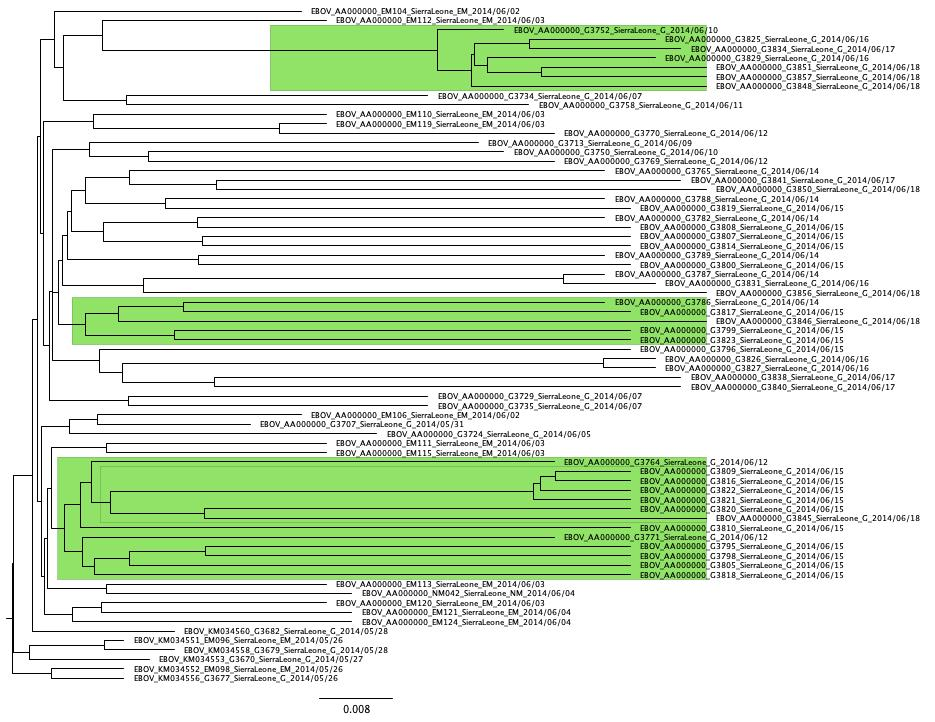
\includegraphics[scale=0.6]{ebola_tree_hl.jpg}
		\caption{Our tree!}
	\end{figure}
	
\section*{Discussion}
	We can infer the start of epidemic to be $\tfrac{0.0824}{1/365} = 30.076 \approx 30$ days before the most recent sample date.
	Since the latest sample was taken on June 18th, then the first incident of the outbreak is estimated to be on May 19th. 
	The interval of 95\% highest posterial density of this parameter is between April 26th and May 26th. 
	
	The \textit{TreeHeight} parameter represents the date of the root or MRCA for the 72 sampled sequences. 
	The mean of the height is $\tfrac{0.0749}{1/365} = 27.338 \approx 27$ days.
	
	In Fig. \ref{fig:Rboxplot}, we can see that the medians of posteriors for reproduction ratios are not extremely different among three values. 
	This is also supported by the skyline we obtained using \texttt{bdskytools} in \texttt{R 3.5.3}. 
	In the analysis, it was difficult to get a smooth skyline plot since the changes among the $R_i$'s are not noticeable.
	
	Through \texttt{Tree Annotator}, from \texttt{BEAST}, we got the phylogenetic tree from 72 sequences of EBOV (Fig. \ref{fig:tree}). 
	The highlighted clades are the most recent samples.  
	
	
	
\printbibliography

\pagebreak
%\section*{Appendix}
%	\begin{figure}[!htbp]
%	\label{fig:sitemodel}
%	\centering
%	\includegraphics[scale=0.4]{sitemodel.png}
%	\caption{Site model option in BEAUTi}
%\end{figure}

%\begin{figure}[!htbp]
%	\label{fig:init}
%	\centering
%	\includegraphics[scale=0.4]{init.png}
%	\caption{Reproduction ratio initialization in BEAUTi}
%\end{figure}

%\begin{figure}[!htbp]
%	\label{fig:prior}
%	\centering
%	\includegraphics[scale=0.4]{priors.png}
%	\caption{Priors setting in BEAUTi}
%\end{figure}

\end{document}

